\chapter{Revisão de Literatura}

Este capítulo aborda os conceitos fundamentais relacionados ao presente trabalho. Na Seção 2.1
são apresentados os principais conceitos referentes a virtualização baseada em contêineres, em seguida, na Seção 2.2 é realizada uma revisão sobre os componentes principais do \textit{Kubernetes}. Logo, na Seção 2.3 é introduzido o tema microsserviços, e na Seção 2.4 é apresentada uma revisão acerca do tema escalonamento de tarefas. A Seção 2.5 apresenta os trabalhos relacionados ao passo que a Seção 2.6 as considerações finais do capítulo.

\section {Computação em Nuvem}
Há muitas definições formais para o termo Computação em Nuvem. A definição internacionalmente proposta pelo \textit{NIST} (\textit{National Institute of Standards and Technology})\cite{mell2011nist} visa o acesso compartilhado, isolado e sob-demanda para um ambiente de recursos computacionais (\textit{e.g.}, redes, servidores, discos, aplicações e serviços). Nesse contexto, os recursos de computação são agrupados e isolados para atender multiusuários. Ou seja, usuários isolados que compartilham recursos computacionais, os quais são dinamicamente provisionados conforme a demanda. Nesse formato há a exigência de rápido ajuste dos recursos elásticos de acordo com a necessidade \cite{Bersten2014}.

\subsection{Virtualização e Nuvem}
A virtualização é considerada uma técnica que permite criar ambientes simulados a partir de um único sistema, seja ele físico ou não. Dessa forma, classifica-se virtualização como tecnologia, enquanto que Nuvem como um ambiente, conjunto de recursos computacionais gerenciável, que pode ou não manipular virtualização \cite{Redhat-virtualization-vs-cloud}. Nos dias atuais, a virtualização de recursos é um dos pontos chaves das Nuvens modernas, a partir da virtualização as Nuvens são capazes de gerenciar ambientes elásticos, que compartilham recursos computacionais isolados logicamente \cite{Zhang2010}. Portanto, Virtualização e Nuvem não são sinônimos.

A virtualização convencional é a baseada na execução de um hipervisor no topo de uma máquina física. Um hipervisor é um software que cria e executa \ac{VM}. Ao utilizar hipervisor o administrador é capaz de otimizar o uso de recursos físicos e modular partes individuais da infraestrutura no formato de \ac{VM}. Assim, os recursos são consumidos com mais eficiência na arquitetura hipervisor quando comparado com implantações \textit{bare-metal} (direto em \textit{hardware}). Em contrapartida, apesar da otimização em relação ao \textit{bare-metal}, o hipervisor executa múltiplos \textit{kernels} em uma única máquina física, tornando custoso o isolamento das aplicações e processos \cite{scheepers2014virtualization}.
%
O presente trabalho não realizará revisão completa sobre virtualização em nuvem, uma vez que na literatura são encontrado diversos trabalhos exploratórios acerca do assunto \cite{Assuno}, \cite{lu2014cloud}, \cite{aceto2013cloud}

\subsection{Contêineres}
Na contemporaneidade, os contêineres são considerados a abordagem padrão para executar cargas de trabalho nas Nuvens Computacionais. No contexto do presente trabalho, um contêiner reflete em uma unidade computacional, que é responsável por executar aplicações. Para gerenciamento de contêineres existem diferentes orquestradores, como por exemplo, \textit{Kubernetes} e \textit{Docker Swarm}.
%
Um contêiner compreende em um conjunto de um ou mais processos dispostos de forma isolada do \ac{SO} hospedeiro. Todas dependências que são necessárias para execução do contêiner são fornecidos por uma imagem distinta. Para a maioria dos motores de contêineres, a imagem representa os passos necessários para construção de um contêiner. A virtualização baseada em contêineres (conteinerização) é considerada uma solução portável, pois permite executar o mesmo contêiner em implantações distintas. Portanto, os contêineres são ideais para encapsular aplicações, migrá-las para hospedeiros distintos sem maiores impasses, e implantar em Nuvem \cite{Redhat-lxc}.

Na literatura há diversas comparações entre contêineres e \ac{VM}, considerando aspectos como desempenho, uso de recursos e segurança. O contêiner é um processo que utiliza o mesmo \textit{kernel} que o \ac{SO} hospedeiro. Já as \ac{VM} simulam um \ac{SO} pleno. Outro ponto a destacar, por convenção, o tamanho de um contêiner é mensurado em \textit{megabytes}, já a \ac{VM} em \textit{gigabyte}. Além disso, nota-se uma tendência de utilizar contêineres para construção de sistemas baseado em microsserviços. Os principais fatores para essa associação são que os contêineres se enquadram no fluxo de desenvolvimento e implantação em Nuvem, são mais leves, e possuem tempo de construção e inicialização inferiores as tradicionais \ac{VM}.

Tanto a conteinerização quanto a virtualização por hipervisor são soluções utilizadas para a implantação de \ac{SAAS} em Nuvem. Entretanto, ao passar do tempo, a conteinerização se tornará um padrão para construção de \ac{SAAS} com características escaláveis, já as \ac{VM} irão continuar com papel importante no provisionamento de \ac{SO} sob-demanda e no fornecimento de \ac{PAAS}.
%
As tecnologias de conteinerização são consideradas um ecossistema que fornecem ferramentas para a conteinerização. Esse ecossistema é composto por Contêiner de Aplicação, Contêiner de Sistema, Gerenciador de Contêiner e Orquestrador de Contêineres. Nessa seção serão explanados os dois primeiros sistemas, enquanto que Orquestrador de contêineres será explicado na seção 2.2.

\subsection{Contêiner de Aplicação e Contêiner de Sistema}
Apesar de se basearem nas mesmas tecnologias e conceitos, há uma diferença clara entre Contêiner de Aplicação e Contêiner de Sistema, e está relacionada ao seu uso. Contêiner de Sistema visa a execução de um \ac{SO} completo, e o Contêiner de Aplicação é designado à implantação de uma aplicação ou de um componente de uma aplicação \newline \cite{casalicchio2020state}. Contêiner de Aplicação refere-se a um contêiner cujo único encargo é executar uma única aplicação dentro de um ambiente isolado. Entretanto, há a possibilidade de utilizar Contêiner de Aplicação como Contêiner de Sistema, mas esse comportamento não está de acordo com \textit{Docker development guidelines and best practices} \cite{berg2016guidelines}, pois Contêiner de Aplicação são designados para executar aplicações no formato de microsserviços. Diferente dos Contêiner de Sistema que são projetados para, em nível de comparação, executar um \ac{SO} de forma similar às \ac{VM}. Um exemplo de Contêiner de Aplicação é o \textit{Docker}, um exemplo de Contêiner de Sistema é o \textit{Linux Containers (LXD)}.

%%\subsection{\textit{Docker}}

%%Segundo \cite{Redhat}, o \textit{Docker} se resume em conjunto de tecnologias, as quais incluem projetos \textit{Open Source}, ferramentas que resultaram desses projeto, e a empresa \textit{Docker Inc}. Em resumo, o termo \textit{Docker} é uma ferramenta de conteinerização para gerenciamento, criação e uso de contêineres \textit{Linux}. Com o \textit{Docker} é possível provisionar contêineres como fossem aplicações isoladas elásticas e extremamente leves.

%%Docker é uma plataforma de código aberto, desenvolvido na linguagen \textit{Go} pela \textit{Google}. 

\subsection{Gerenciadores de Contêiner de Aplicação}
O Gerenciador de Contêiner de Aplicação é considerado um \textit{framework} que fornece ferramentas que auxiliam no gerenciamento de todo o ciclo de vida do contêiner. O ciclo de vida de um contêiner, desde o desenvolvimento até execução em ambiente de produção, de acordo com \textit{IBM} \cite{ibm-ciclo}, compreende em:

\subparagraph{Obtenção:}
Aquisição da imagem do contêiner. Essa etapa é considerada o ponto inicial para a criação de um novo contêiner. Em contêineres \textit{Docker} há a concepção de camadas de imagens, significa que uma imagem pode ser derivada de outras imagens.
\subparagraph{Construção:}
Em \textit{Docker} há um arquivo de definição chamado \textit{Dockerfile}, nele são definidas todas as dependências e a maneira que a aplicação será executada. Normalmente, em um arquivo \textit{Dockerfile} há a escolha da imagem base, passos para montagem do contêiner, e um ponto de entrada para execução de um processo principal (comumente são utilizados processos em segundo plano). Para que ocorra a construção do contêiner com sucesso, todos os passos de montagem devem ser executados com êxito.
\subparagraph{Entrega:}
Na entrega é definido um \textit{pipeline} de verificações do contêiner. O \textit{pipeline} geralmente executa os testes da aplicação e verifica vulnerabilidades, ao passar por todas as checagens o contêiner é entregue para o ambiente de produção.
\subparagraph{Implantação:}
A Implantação representa os passos para que um novo contêiner seja executado em ambiente de produção. Nesta etapa é feito a substituição da imagem do contêiner em execução, para isso é necessário algum sistema que faça esse controle.
 
\subparagraph{Execução:}
Nessa etapa é definido o ambiente de execução do contêiner, que pode envolver: dimensionamento da aplicação por meio de réplicas, verificação de falhas e conexão com outros serviços e réplicas.

\subparagraph{Gerenciamento:}
O passo final refere-se ao gerenciamento da aplicação conteinerizada em ambiente de produção. Nessa fase, a aplicação pode estar em execução ou em suspensão. Em gerenciamento, o comportamento da aplicação é monitorado, o sistema deve ser capaz de gerenciar as falhas nos contêineres que estão em execução, por exemplo, forçando a reinicialização. Enquanto que a suspensão é um estado para depuração da aplicação, com o objetivo de encontrar a origem da falha. Posteriormente, o processo passa por todas as fases novamente, iniciando em Obtenção.

Gerenciadores de Contêineres são classificados em auto-hospedados ou baseados em soluções gerenciadas. Soluções auto-hospedadas percorrem todo o ciclo de implementação de um Gerenciador de Contêiner de Aplicação: instalação, configuração e gerenciamento em \textit{datacenters} privados, máquinas virtuais ou até mesmo em \textit{clouds} geograficamente distribuídas. Por outro lado, soluções gerenciadas são ofertadas por provedores de nuvem e necessitam apenas de configuração parcial \cite{casalicchio2020state}. Assim, as plataformas de conteinerização \textit{Docker, LXD, OpenVZ} podem ser configuradas da mesma maneira que Gerenciadores de Contêiner de Aplicação, portanto, são exemplos de soluções auto-hospedas. Os exemplos mais populares de soluções gerenciadas são das empresas \textit{Google} e \textit{Amazon} que possuem serviços como, respectivamente, \textit{GKE} (\textit{Google Kubernetes Engine}) e \textit{EKS} (\textit{Elastic Kubernetes Service}).

\section{\textit{Kubernetes}}
Para \citeonline{Arundel}, o \textit{Kubernetes} é considerado o Sistema Operacional das Nuvens Computacionais, sendo o sistema de orquestração de contêineres padrão no mercado. Para isso, o \textit{Kubernetes} oferece um ambiente robusto para implantação de sistemas voltados para nuvem. As principais características do orquestrador são: escala automática de cargas de trabalho por meio de réplicas, balanceamento de carga, escalonamento por agrupamento ou espalhamento, e monitoramento do \textit{cluster}.

O \textit{Kubernetes} é um sistema de orquestração que agrupa contêineres em \textit{pods}. \textit{Pod} é um grupo com um ou mais contêineres que compartilham recursos de armazenamento e rede. Dessa forma, contêineres dispostos em um mesmo \textit{pod} são escalonados e executados juntos \cite{Google}. Ou seja, todas as dependências que a aplicação conteinerizada necessita serão lançadas e agrupadas ao mesmo tempo e \textit{pod}, respectivamente. Além disso, a \textit{Google} disponibiliza, de forma oficial, bibliotecas que utilizam API \textit{(Application Programming Interface)} do \textit{cluster} \textit{Kubernetes}  para as principais linguagens de programação (\textit{e.g.}, \textit{.NET}, \textit{Python}, \textit{Java}, \textit{Go}, \textit{JavaScript}, \textit{Haskell}). Por meio da API é possível obter o estado do \textit{cluster}, configurar, lançar e escalonar \textit{pods} no \textit{Kubernetes} \cite{KubernetesAPI}.

\subsection{Componentes \textit{Kubernetes}}
Um \textit{cluster} \textit{Kubernetes} consiste em um conjunto de servidores, chamados de \textit{nodes}, que executam serviços conteinerizados. O sistema principal do \textit{Kubernetes} é o \textit{Control Plane}, que é responsável por tomada de decisões, escalonamento e controle do estado do \textit{cluster}. O \textit{Control Plane} reside em um \textit{node} específico denominado \textit{Master} e consiste em cinco componentes:

\begin{itemize}
    \item \textit{Kube-apiserver}: Servidor \textit{frontend} para o \textit{Control Plane}, trata requisições que são direcionadas à \textit{API} do \textit{Kubernetes};
    \item \textit{Etcd}: Banco de dados, do tipo \textit{chave-valor}, que armazena informações sobre o estado do \textit{cluster};
    \item \textit{Kube-scheduler}: Componente responsável por observar novos \textit{pods} e escaloná-los em um \textit{node};
    \item \textit{Kube-controller-manager}: Executa os controladores de recurso, que incluem: Controlador de \textit{nodes}, Controlador de Réplicas, Controlador de Autenticação. Este componente é responsável verificar o estado do \textit{cluster}, das cargas de trabalho e serviços, com objetivo de mover o estado atual para o estado desejado.
    \item \textit{Cloud-controller-manager}: Responsável por gerenciar a interação com o provedor de Nuvem.
\end{itemize}

O diagrama de um \textit{cluster kubernetes} com todos os componentes interligados é visualizado na Figura \ref{fig:components_of_kubernetes}.
%
O exemplo é composto por três \textit{nodes} gerenciados pelo \textit{Control Plane}.
%
Destaca-se a presença do \textit{sched}, ou seja, o escalonador responsável por selecionar os hospedeiros para os contêineres.

\begin{figure}[h!]
	\caption{\label{fig:components_of_kubernetes}Componentes \textit{cluster Kubernetes}}
	\centering
	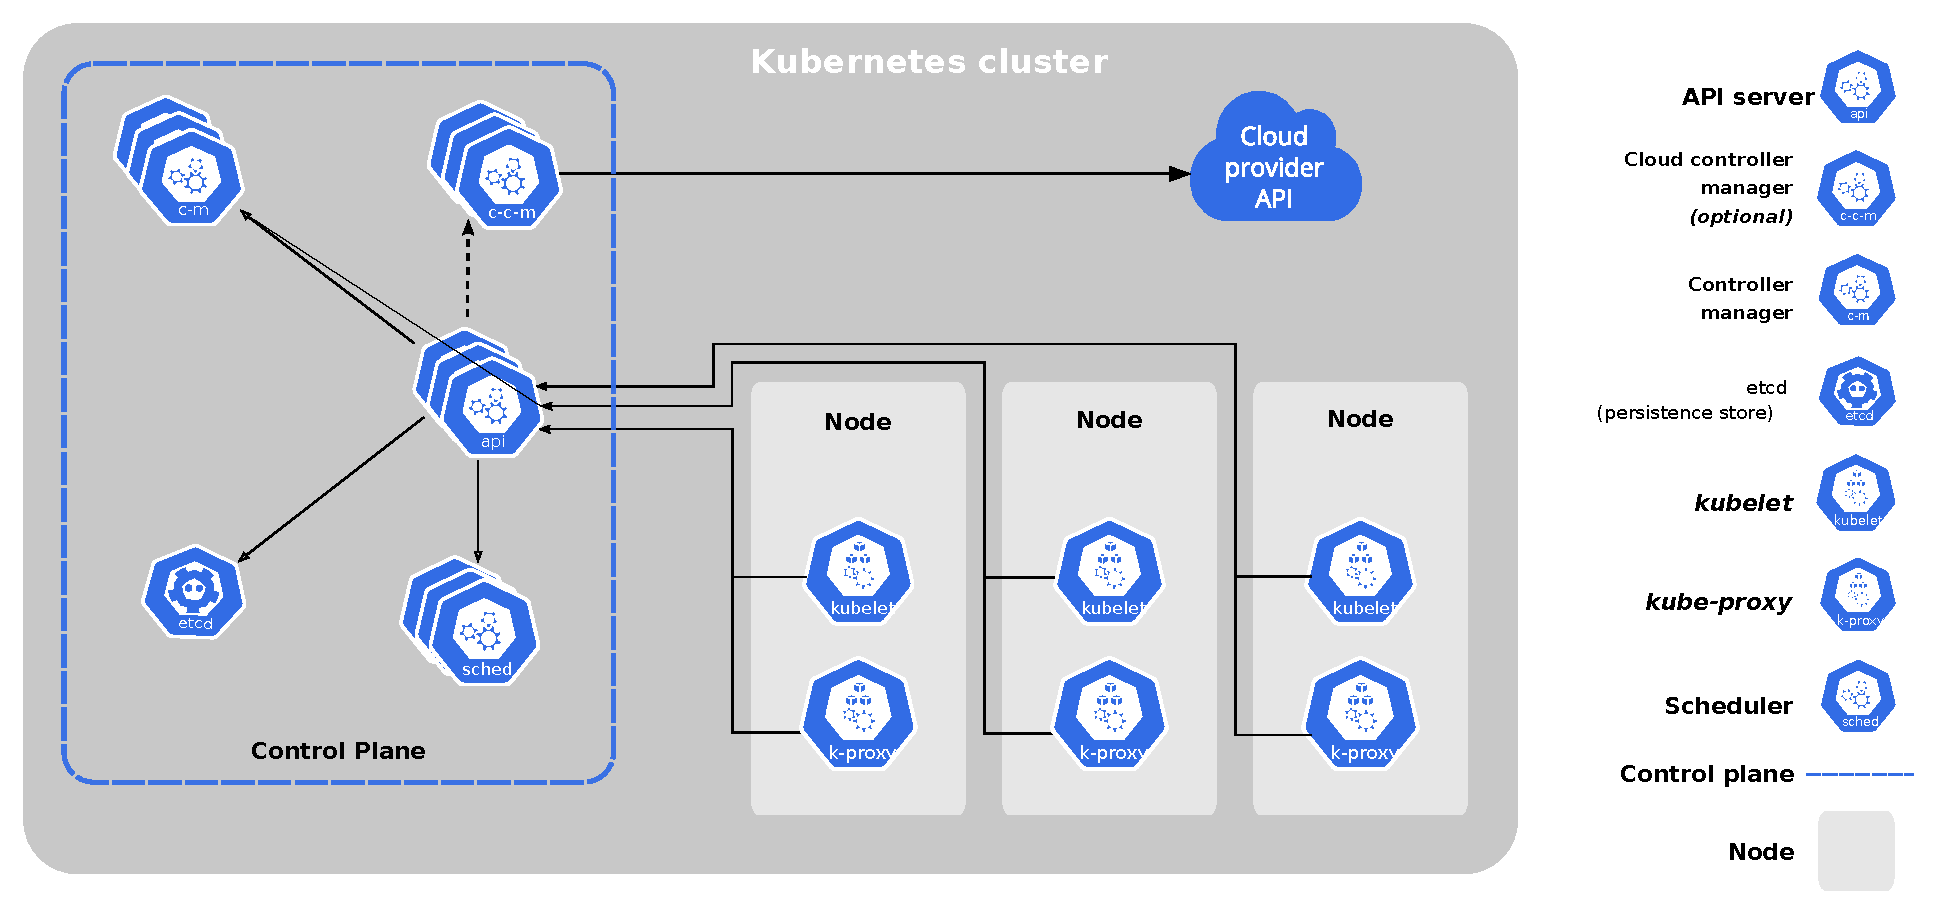
\includegraphics[width=.84\linewidth]{assets/components-of-kubernetes.pdf}
	\legend{Fonte: \citeonline{kubernetesCoreComponentes}}
\end{figure}

\newpage
\subsection{Objetos e serviços Kubernetes}
Além dos componentes do \textit{Control Plane} existem outros objetos e serviços que são fundamentais para a conteinerização, funcionamento do \textit{Kubernetes}, ou são pertinentes a este trabalho. 

\subparagraph{\textit{Pods}:} representa a menor unidade de objeto no \textit{Kubernetes}. Em resumo um \textit{pod} é uma carga de trabalho que é executada em \textit{nodes} do \textit{cluster} no formato de um processo.
\textit{Pod} é considerado um grupo com um ou mais contêineres, os quais compartilham recursos de disco e rede. 
Cada \textit{pod} contém especificação declarativa da execução dos contêineres que possui. A comunicação entre os contêineres de um mesmo \textit{pod} é feita por meio de \textit{inter-process comunication (IPC)}, como semáforos \textit{SystemV}, ou, utilizando a memória compartilhada \textit{POSIX}. Por padrão, contêineres em \textit{pods} distintos não se comunicam por meio de \textit{IPC} sem configuração personalizada. Desse modo, a comunicação entre contêineres em \textit{pods} distintos é concebida via troca de mensagem utilizando protocolo \textit{IP}.
	
\subparagraph{\textit{ReplicaSet}:}
Considerado um serviço responsável pelo controle de réplicas de \textit{pods} solicitado. Assim, o \textit{ReplicaSet} garante a disponibilidade de um número de \textit{pods}.
	
\subparagraph{\textit{Deployments}:}
fornece atualizações declarativas para \textit{pods} e \textit{replicaSets}. Ou seja, o \textit{deployment} é usado para atualização de estado de \textit{pods} e \textit{ReplicaSets}. O uso comum de \textit{deployments} em relação ao \textit{pod} é na atualização de imagem do contêiner, já para \textit{ReplicaSet} seria na atualização no número de réplicas disponíveis desejado.

\subsection{Detalhes de escalonamento}
Para realizar o escalonamento dos \textit{pods}, o \textit{kube-scheduler} executa um fluxo de operações que são separadas em duas categorias: Filtragem e Ranqueamento. Em resumo, a filtragem consiste em investigar \textit{nodes} que são capazes de executar o \textit{pod} a ser escalonado, ou seja, nessa etapa há a seleção dos \textit{nodes} do \textit{cluster} que satisfazem a solicitação de recursos do \textit{pod}. O ranqueamento, por sua vez, classifica os \textit{nodes} eleitos pela filtragem e seleciona o \textit{node} que obter a maior pontuação de acordo a solicitação de recursos do \textit{pod} \cite{Kubescheduler}.

A técnica de escalonamento utilizada pelo \textit{kube-scheduler} é denominada \textit{First-Come-First-Served} (FCFS), conhecida também como \textit{First-In-First-Out} (FIFO), que consiste em escalonar os serviços pela ordem de chegada. Alguns motivos são elencados para defender a escolha dessa técnica, por exemplo, garantia da ausência de inanição e simples implementação algorítmica. Embora exista o consenso que há espaço de melhoria, substituir essa técnica de escalonamento por um algoritmo aprimorado 
requer um estudo de caso específico bem definido \cite{CarastanSantos2019}.

\subsection{Customização do \textit{kube-scheduler}}
\label{customizacao_kube_scheduler}
De acordo com \citeonline{ibm-sched} há 4 meios de customizar o escalonador do \textit{Kubernetes}, que serão abordados nessa seção.

\subparagraph{Alteração do código fonte:}
A primeira técnica consiste em clonar o repositório do código fonte do \textit{Kubernetes}, modificar o comportamento do escalonador padrão, recompilar o projeto e executar o escalonador. Essa prática não é recomendada pois há a necessidade de alinhar o código alterado com o fluxo de execução do \textit{Kubernetes}. O segundo fator que desmotiva esse método, é que o próprio \textit{Kubernetes} oferece meios para alterar o comportamento do escalonador sem a necessidade de alterar o código fonte.

\subparagraph{Extensão do escalonador padrão:}
A segunda solução é denominada Extensão, considerada a solução mais simples, que objetiva adicionar funcionalidades extras ao \textit{kube-scheduler}. Extensão é entendido como a configuração de ganchos (\textit{webhooks}) que o \textit{Kubernetes} oferece para executar filtragem e ranqueamento dos \textit{nodes} de forma customizada. Ganchos devem ser interpretados como gatilhos, que são funções personalizadas que o \textit{Kubernetes} invoca para alterar algum comportamento padrão ou adicionar novas funcionalidades. Embora seja simples implementação, essa técnica possui uma limitação que não a permite que seja usada no presente trabalho, os únicos pontos de extensão do escalonador são apenas nos procedimentos das fases de filtragem e ranqueamento, não atuando no início nem no fim de nenhuma outra etapa de escalonamento. 

\subparagraph{\textit{Framework} de escalonamento:}
O terceiro método para customizar o escalonador padrão do \textit{Kubernetes} é denominado \textit{framework} de escalonamento. Essa técnica consiste em adicionar pontos de extensão no escalonador padrão do \textit{Kubernetes}, chamados \textit{plugins}, que são incluídos em tempo de compilação. Os \textit{plugins} podem ser habilitados, desabilitados e reordenados. \textit{Plugins} são adicionados nos ciclos padrões de escalonamento -- \textit{scheduling} e \textit{binding}. No ciclo \textit{scheduling} está habilitada a extensão por meio de 8 \textit{plugins}: \textit{sort, PreFilter, Filter, PreScore, Score, NormalizeScore, Reserve, Permit}. Já, na fase de \textit{binding} há 3 pontos de extensão: \textit{PreBind, Bind, PostBind}. O presente trabalho não realizará revisão completa sobre os pontos de extensão, uma vez que a documentação explora este assunto de forma ampla \cite{schedulerframework}. Essa técnica é considerada uma ampliação da Extensão do escalonador, entretanto, necessita exige que a implementação seja feita na linguagem \textit{Go} para que o \textit{plugin} seja compilado e executado pelo escalonador padrão do \textit{Kubernetes}.

\subparagraph{Múltiplos escalonadores:}
A quarta técnica é executar um escalonador customizado ao lado do escalonador padrão. O escalonador customizado é conteinerizado no formato de \textit{pod} e orquestrado pelo próprio \textit{Kubernetes}. Nessa abordagem, as informações pertinentes ao escalonamento (estado do \textit{cluster} e lista de \textit{pods}) são coletadas pela \textit{Kube API}. Para que o escalonador padrão e o customizado não disputem os mesmos \textit{pods}, na criação de novos \textit{pods} é preciso identificar o método de escalonamento por meio do nome do escalonador. Caso contrário, a coexistência de múltiplos escalonadores causa o bloqueio de sincronização.
%A comunicação do \textit{pod}, abstraído em escalonador de contêineres, com a \textit{API} do \textit{Kubernetes} é custosa. Pois o \textit{pod} irá consumir a \textit{API} do \textit{Kubernetes} por meio do protocolo \ac{HTTP}.

Portanto há 4 maneiras de customizar o escalonamento no \textit{Kubernetes}, desde uma técnica simples para pequenas alterações até a construção de um \textit{plugin} compilado no escalonador padrão, respectivamente Extensão do Escalonador Padrão e \textit{Framework} de escalonamento. No escopo desse trabalho, a principal desmotivação ao usar essas duas técnicas é que são apoiadas pelo escalonador padrão, que em cenários de falhas o processo de escalonamento é interrompido até a reinicialização do escalonador. Visando desenvolver um sistema distribuído, a técnica escolhida para o projeto é a Múltiplos escalonadores, que permite desenvolver um escalonador em qualquer tecnologia/arquitetura desde que se comunique com a \textit{Kube API}.

%\textcolor{red}{TODO: qual voce usará? Deixe claro aqui.}

\subsection{Alta disponibilidade}
A configuração de um \textit{cluster} \textit{Kubernetes} visando alta disponibilidade é essencial para o uso de aplicações conteinerizadas em produção. A alta disponibilidade é alcançada a partir da replicação do \textit{node} \textit{master}, com isso, eliminando um único ponto de falha para os componentes do \textit{Control Plane}, que são fundamentais para o funcionamento do \textit{Kubernetes} \cite{Kubeha}.

A implantação do \textit{Kubernetes} com a configuração padrão de alta disponibilidade consiste em replicar os componentes do \textit{Control Plane}. A instância do banco de dados \textit{etcd} será replicada utilizando um algoritmo de consenso e todos os servidores \textit{Kube-apiserver} estarão disponíveis por meio de um balanceador de carga. Na mesma linha de pensamento, os demais componentes (\textit{Kube-controller-manager}, \textit{Cloud-controller-manager}, \textit{Kube-scheduler}) estarão com réplicas em estado de espera aguardando alguma falha acontecer na instância primária. Um exemplo de ambiente \textit{Kubernetes} em alta disponibilidade é visto na Figura \ref{fig:components_of_kubernetes_ha}.


\begin{figure}[h!]
	\caption{\label{fig:components_of_kubernetes_ha}Componentes \textit{cluster Kubernetes} com alta disponibilidade}
	\centering
	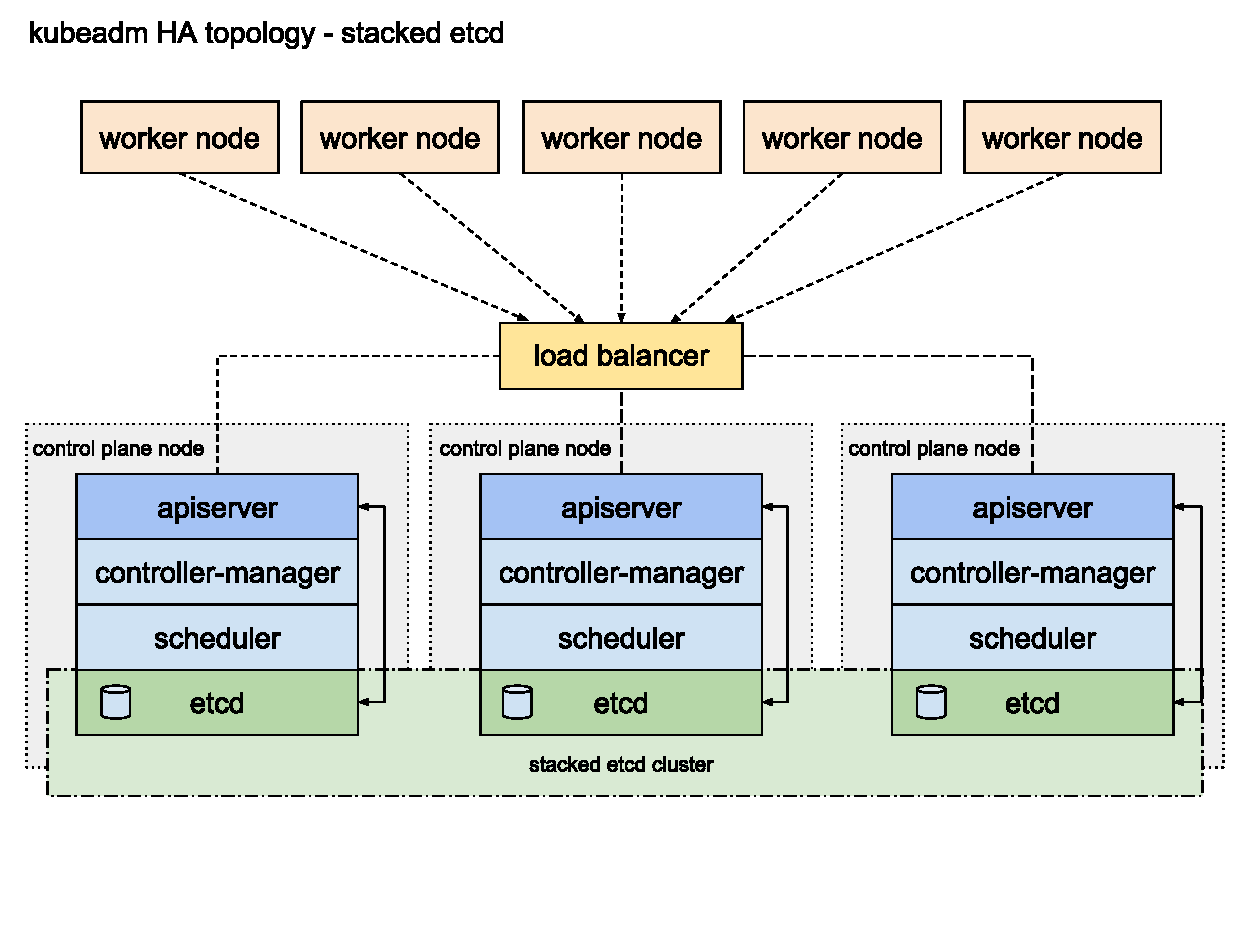
\includegraphics[width=.84\linewidth]{assets/components-of-kubernetes-ha.pdf}
	\legend{Fonte: \citeonline{kubernetesCoreComponentes}}
\end{figure}

A replicação dos componentes do \textit{Control Plane} é uma solução sólida para tolerância a falhas, contudo, há espaço de melhoria no processo escalonamento. A razão é que as réplicas do \textit{Kube-scheduler} não atuam em conjunto nesse processo, ou seja, no momento em que a instância primária falhar haverá um período de tempo até a réplica iniciar a execução do escalonamento. Essa janela de tempo entre a falha da instância padrão até a réplica começar a trabalhar reflete diretamente na degradação do tempo de espera de escalonamento. A solução do presente trabalho é distribuir o processo de escalonamento em réplicas ativas, para que em cenários de falhas se consiga trabalhar com uma boa margem de tempo de espera. A execução do algoritmo será apresentada no Capítulo \ref{cap-proposta}.

\section{Microsserviços}

De acordo com \citeonline{FowlerMicrosservice} não há definição precisa de microsserviços, contudo, existem algumas características em comum acerca das implantações dessa arquitetura. Como por exemplo, um conjunto de serviços que constitui um sistema, controle descentralizado da informação, automação da implantação de \textit{software} e uso heterogêneo de linguagens de programação e banco de dados.
Detalhes sobre definições e conceitos de microsserviços são revisados na presente seção, uma vez que o presente trabalho utilizará tal abordagem para implementação do escalonador.

\subsection{Definições e conceitos}
A arquitetura de microsserviços visa o desenvolvimento de um sistema como um conjunto de serviços sucintos seccionados em processos independentes, podendo ou não compartilhar o mesmo hospedeiro \cite{lewis2012microservices}. Isto é, microsserviços são pequenas aplicações que podem ser implantadas, escaladas e testadas independentemente, que possuem um conjunto limitado de funcionalidades para resolver um só objetivo. Uma única responsabilidade, por um lado, deve ser interpretada como uma única razão para mudar ou uma única razão para ser substituída. Por outro lado, deve ser interpretada como um sistema que possui uma funcionalidade apenas, o qual tem de ser facilmente  compreendido fora de seu contexto. Considera-se que o conceito de microsserviço está relacionado com a filosofia \textit{unix}: Escreva programas que façam apenas uma coisa, mas que façam bem feita e Escreva programas que trabalhem juntos \cite{thones2015microservices}.

%Para a interação entre os serviços que compõe um sistema, os microsserviços se beneficiam de protocolos leves para troca de mensagem, como \ac{RPC}, protocolo de mensagens e, se for necessário, é possível utilizar \ac{HTTP}~\cite{ericraymond2003}.

%. O \ac{HTTP} é a forma habitual  que o navegador carrega páginas da \ac{WWW}, enquanto que, \ac{RPC} e fila de mensagens são protocolos comumente empregado para comunicação de sistemas distribuídos 

\subsection{Do monolítico ao microsserviços}
Em engenharia de \textit{software}, um sistema monolítico constitui-se de uma única unidade, ou seja, todo código é vinculado a um único processo. Aplicações comerciais geralmente são divididas em três partes: lado cliente, habitualmente uma página \textit{web}, banco de dados e uma aplicação do lado servidor. Em uma aplicação \textit{web}, esse servidor lida com o \ac{HTTP}, executa a regra de domínio e persiste informações no banco de dados. O sistema do lado servidor é considerado monolítico. Por consequência, qualquer alteração no sistema influenciará em construir e implantar uma nova versão da aplicação.

Desenvolver de forma monolítica é a maneira natural de construir sistemas, sendo que toda a lógica é gerenciada por um único processo. O projeto para esse tipo de sistema equivale a segregar as partes/módulos do sistema por meio das técnicas de programação da linguagem utilizada, por exemplo classes, interfaces, hierarquia, etc. Entretanto, sistemas monolíticos não oferecem escalabilidade, pois escalar tal sistema consiste em replicar o sistema de forma integral. 
Por sua vez, uma aplicação baseada em microsserviços proporciona um escalabilidade inteligente, pois replica as partes de acordo com a necessidade por meio de um balanceador de carga dedicado para cada serviço, como ilustra a Figura~\ref{monolitico-microsservico}.

\begin{figure}[ht!]
    \caption{\label{monolitico-microsservico}Comparação entre Monolítico e Microsserviços}
    \centering
    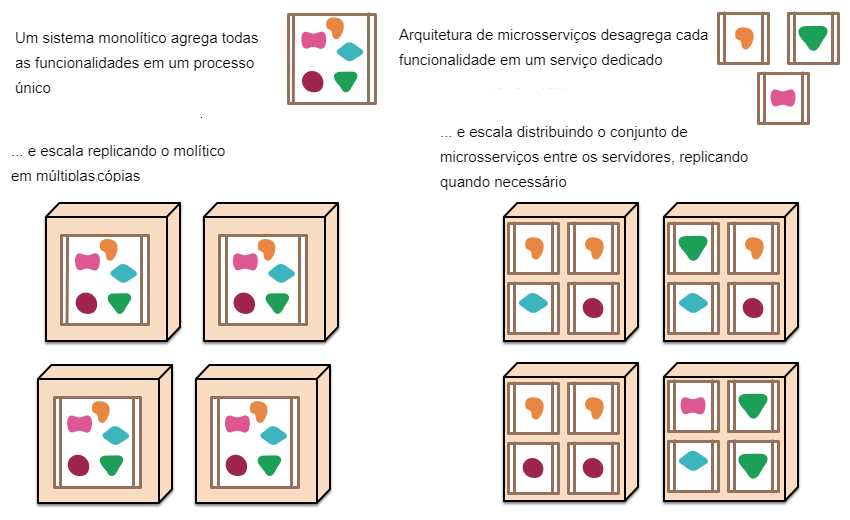
\includegraphics[width=0.85\linewidth]{assets/monilitico-microsservico.png}
    \legend{Fonte: \citeonline{FowlerMicrosservice}}
\end{figure}

\subsection{Projeto de Microsserviço guiado pelo \textit{DDD}}
O \ac{DDD}, no contexto de engenharia de \textit{software}, é uma metodologia que conecta conceitos de linguagem de programação, por exemplo nomes de classes, métodos, e atributos, com o domínio do negócio \cite{DDD}. Define-se domínio como a área de conhecimento, ou seja, as funcionalidades do sistema a nível de negócio \cite{evans2014domain}.
%
De acordo com \citeonline{FowlerMicrosservice}, o \ac{DDD} decompõe um domínio complexo em múltiplas partes, sendo definido na literatura como contextos delimitados (\textit{bounded context}), como também visa o projeto do relacionamento entre esses. Este padrão é utilizado tanto para projetar sistemas monolíticos quanto distribuídos em microsserviços. 
%Nota-se uma correlação semântica entre um serviço e um contexto delimitado, que reforça a separação lógica do domínio em serviços isolados, consequentemente, em microsserviços. Isto é, o contexto delimitado do conceito do \ac{DDD} se torna um excelente candidato à um microsserviço \cite{newman2015building}. Contudo, nem todo contexto delimitado deve ser relacionado à um microsserviço independente. Segundo o criador do \ac{DDD}, Eric Evans, há diferentes tipos de contexto delimitado que não mapeiam diretamente a um serviço isolado.
Um dos desafios de projetar sistemas baseados em serviços distribuídos é determinar a granularidade em termos de escopo e complexidade do microsserviço. O conjunto de funções que definem o microsserviço não deve ser extremamente simplista, muito menos agregar muita complexidade \cite{merson2020modeling}. Portanto, para permitir o gerenciamento descentralizado de acordo com o contexto do domínio, o ideal é unir os princípios do \ac{DDD} com a arquitetura de microsserviços.
%
Tal abordagem é seguida na presente proposta de escalonamento de contêineres, formalmente descrita no Capítulo~3.

\section{Escalonamento de Contêineres}

O escalonamento consiste em um processo de tomada de decisão, que é usado regularmente no ramo da manufatura, serviços industriais e sistemas operacionais. O escalonamento lida com alocação de recursos para tarefas em determinados períodos de tempo, visando otimizar um ou mais objetivos \cite{pinedo2012scheduling}. Alguns desses objetivos, são, redução do tempo de espera das tarefas, maximização do uso de recursos (espalhamento), ou minimização do uso total de recursos (agrupamento).

Neste trabalho, escalonamento é um procedimento que soluciona as alocações de recursos computacionais. Recursos refletem em quantidade mensurável de memória, processamento e dispositivos de rede de um ou mais nós computacionais  (também denominado por máquinas). Formalmente, segundo \citeonline{brucker1999resource}, $m$ máquinas $M_j (j = 1, \dots, m)$ devem processar $n$ trabalhos $J_i (i = 1, \dots, n)$. 
Vinculado a cada trabalho $J_i$ há um número $t_i$ de tarefas $(O_{i1}, O_{i2}, \dots, O_{it_i})$, e para cada tarefa há uma solicitação de recursos $p_{ik}$. 
Dessa forma, o escalonamento é um processo de tomada de decisão que, a partir da requisição de recursos das tarefas,  investigará os nós computacionais  factíveis e indicará o escalonamento ideal de $J_i$ para $M_j$ de acordo com a otimização de alguma métrica de interesse. Um escalonamento válido para alocação de trabalhos pode ser representado por meio do diagrama de Gantt, como exemplifica a Figura \ref{gantt-schedulling}. No exemplo da figura, há o escalonamento de 4 \textit{jobs} para 5 máquinas, os índices se repetem pois se trata de um escalonamento de \textit{jobs} preemptivos.

%\textcolor{red}{TODO: explique a figura. Por qual motivo repete os índices dos jobs??? Explique o que está desenhado.}

\begin{figure}[ht!]
    \caption{\label{gantt-schedulling}Visualização escalonamento por meio do diagrama de Gantt}
    \centering
    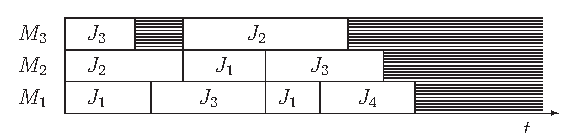
\includegraphics[width=\linewidth]{assets/gantt-scheduling.pdf}
    \legend{Fonte: \citeonline{brucker1999resource}}
\end{figure}

De acordo com \cite{pinedo2012scheduling}, o problema de escalonamento é representado por uma tripla $\alpha|\beta|\gamma$. O campo $\alpha$ representa o ambiente, interpreta-se como o perfil da arquitetura que detém os recursos em que os trabalhos serão escalonados. O campo $\beta$ define detalhes de processamento e restrições que estão vinculados ao trabalho, pode conter nenhuma, uma única ou várias entradas. Já o campo $\gamma$ descreve a função objetivo a qual visa otimização de alguma métrica de interesse, normalmente contém apenas uma entrada.

Para este trabalho, a entrada $\gamma$ será definida pelo perfil \textbf{Máquinas em Paralelo com Diferentes Velocidades} e é representado pelo rótulo $Qm$. Este cenário consiste em $m$ máquinas heterogêneas, que não necessariamente possuem a mesma quantidade de recursos. Considera-se a principal abordagem das nuvens computacionais atualmente \cite{krauter2002taxonomy}.

A entrada $\beta$ é definida pelo conjunto \textbf{Prazo ou \textit{deadline}} ($P$), \textbf{Restrição de Elegibilidade} ($M$) e \textbf{Processamento em Lote} ($batch(b)$). Se o rótulo $P$ está presente em $\beta$, então para cada trabalho $J_{k}$ será atribuído um prazo de entrega $P_{k}$, dessa forma, $J_k$ não deve ser escalonado após o prazo $P_{k}$. Se $P$ não está incluído em $\beta$, logo não há restrição de \textit{deadline} de escalonamento. O rótulo $M$ denota que nem todas as máquinas são capazes de processar o trabalho $J_{k}$, assim, o conjunto $M_{k}$ representa as máquinas que satisfazem as restrições de $J_{k}$, que por consequência, são elegíveis ao escalonamento. Por último, se há rótulo $batch(b)$ em $\beta$, então, uma máquina é apta a processar quantidade $b$ de trabalhos de forma simultânea.

Portanto, $\beta=\{P, M, batch(b)\}$. O campo $\gamma$, que está relacionado com métricas de escalonamento e funções objetivos, será desenvolvido na seção subsequente.

\subsection{Métricas de Escalonamento e Função Objetivo}
De acordo com \cite{Feitelson98}, há um conjunto de métricas relevantes a respeito do desempenho de algoritmos de escalonamento. O presente trabalho visa a otimização das seguintes métricas: tempo de espera de escalonamento e \textit{makespan}. Além disso, ocorrerá a análise do comportamento do \textit{slowdown}.

\subsubsection{Tempo de Espera}
Considerando $Submetido_k$ como o momento em que o trabalho $J_k$ foi submetido à plataforma, $Inicio_k$ o momento em que o trabalho $J_k$ iniciou sua execução, a Equação \ref{eq:1} mensura o tempo de espera, ou seja, o tempo que o trabalho permanece na fila até ser escalonado.

\begin{equation} \label{eq:1}
T_k = Inicio_k - Submetido_k
\end{equation}

A minimização do tempo de espera é um objetivo conhecido e importante no fornecimento de \textit{Quality of Service (QoS)} em muitos cenários \cite{Ye2007}. Por ser classificado como um problema \textit{NP-Hard} \cite{Kubiak1993}, na literatura são encontradas diferentes heurísticas que aproximam-se da solução ideal, pois não há algoritmo de busca eficiente que encontre uma sequência ótima.

\subsubsection{\textit{Makespan}}
A próxima métrica a ser considerada é o \textit{makespan}, que é uma métrica diretamente vinculada ao tempo de completude de um trabalho. O cálculo é definido pelo tempo de término da última tarefa de um trabalho a deixar o sistema. Considerando que um trabalho $J_k$ possui $n$ tarefas vinculadas $O_{k,1}, O_{k,2}, ..., O_{k,n}$, e para cada tarefa $O_{k,i}$ há vinculado o tempo de finalização $C_i$, assim o \textit{makespan} $C_{max, k}$ de $J_k$ é calculado de acordo com a Equação~\ref{eq:make}.

\begin{equation} \label{eq:make}
C_{max,k} = max(C_1, C_2, ..., C_n) 
\end{equation}

A minimização do \textit{makespan} resulta na otimização da utilização dos recursos computacionais \cite{pinedo2012scheduling}, pois o \textit{makespan} está relacionado ao tempo que o trabalho permanece na plataforma.
Ainda, a sua minimização acarreta em melhor agrupamento do escalonamento, que por consequência, ocorrendo a liberação do uso de recursos em um menor período de tempo.

\subsubsection{\textit{Slowdown}}
Por último, outra métrica abordada neste trabalho é o \textit{slowdown}, que é definido pela relação entre o tempo total que o trabalho permaneceu na plataforma com o tempo atual de processamento gasto com o mesmo. Assim o \textit{slowdown} $Sd_k$ de $J_k$  é definido pela Equação \ref{eq:2}, sendo que \(P_{k}\) é o tempo de processamento de \(J_k\).

\begin{equation} \label{eq:2}
Sd_{k} = \frac{T_{k} + P_{k}}{P_{k}}
\end{equation}

O propósito do \textit{slowdown} é estabelecer  proporção entre tempo de espera de um trabalho em relação ao seu tempo de processamento \cite{Maccio2018}, com o objetivo de atribuir uma distribuição equilibrada do tempo de espera entre os trabalhos com diferentes cargas de trabalho \cite{CarastanSantos2019}.

\subsubsection{Função Objetivo}
Portanto o campo $\gamma$ (função objetivo) da definição de escalonamento refere-se à minimização do tempo de espera, \textit{makespan}, logo, $\gamma = T, C_{max}$. Em cenários como \ac{HPC}, os resultados visados por meio da otimização desse conjunto de métricas são: obter melhor \textit{QoS} por meio da minimização do tempo de espera; Otimizar a utilização dos recursos computacionais mediante a minimização do \textit{makespan}; e Analisar o comportamento do \textit{slowdown}.

\subsection{Escalonamento Distribuído}

Aplicações atuais fundamentam-se na análise e processamento de um grande volume de dados, como por exemplo, \textit{Data Mining}, \textit{Machine Learning}, \textit{Deep Learning} e bancos de dados. Dessa forma, conforme a demanda de poder computacional cresce, as estruturas responsáveis pela execução dessas aplicações os acompanham, refletindo no aumento de complexidade tanto em tamanho como em algoritmos refinados de gerenciamento \cite{Wang2016LoadbalancedAL}. A nível de comparação desse reflexo, a empresa \textit{Google} executa centenas de milhares de cargas de trabalho, de milhares de aplicativos em um conjunto de \textit{clusters}, cada qual com até dezenas de milhares de máquinas \cite{Google2015Borg}. 
Por consequência, os componentes de gerenciamento de um \textit{data center} de larga escala devem resolver os problemas internos com algoritmos complexos e sofisticados para cada tipo de cenário.

O escalonamento é um tema amplamente pesquisado, desde otimização por meio de processamento em \textit{GPU} \cite{Nesi2018ScheduleGPU} como também baseado em arquitetura descentralizada empregando conceitos de \textit{blockchain} \cite{loch2021novel}. De acordo com a literatura, o escalonamento distribuído é requisito fundamental para \textit{Data Centers} de larga escala \cite{Google2015Borg, Wang2019Pigeon}, uma vez que a principal dificuldade da abordagem centralizada está na escalabilidade e nos métodos de tolerâncias a falhas, que degradam por completo as métricas de \ac{QOS}. O escalonamento, no formato distribuído, resolve este problema de forma elaborada removendo o único ponto de falha ao particionar as requisições de alocação de recursos em um sistema distribuído.

\section{Trabalhos Relacionados}

A área de escalonamento de tarefas realiza a intersecção de diferentes campos da ciência da computação. Um dos principais fatores que impulsionam a intersecção entre as áreas está na natureza do problema de escalonamento, pois resolver um problema de escalonamento reflete em otimizar um problema \textit{NP-difícil}. Dessa forma, na literatura encontram-se diferentes pesquisas que refletem em soluções heurísticas e refinadas, muitas vezes relacionadas com a área de inteligência artificial. Por se tratar da solução de um problema \textit{NP-difícil}, a solução computada basta ser boa o suficiente para um cenário específico, sendo assim, a solução encontrada nem sempre é refletida na ótima global.

Esta seção analisará trabalhos recentes da literatura que possuem relação com escalonamento de contêineres. Por ainda se tratar de um recorte amplo na área de escalonamento, aqui analisaram-se diferentes trabalhos que atacam características distintas, sejam relacionadas com otimização energética em \textit{data centers} como também trabalhos que buscaram otimizar o desempenho de escalonamento.

No trabalho de \citeonline{sureshkumar2017optimizing} os autores propuseram um algoritmo de escalonamento de contêineres, para a tecnologia \textit{Docker}, baseado em balanceamento de carga. O algoritmo consiste em um limiar calculado a partir da sobrecarga do \textit{cluster}.
O objetivo do limiar é que as cargas dos contêineres não sejam altas ou baixas. Quando a carga ultrapassa o limiar, um novo contêiner é criado no balanceamento de carga. Por outro lado, quando a carga é muito baixa, o contêiner é destruído com o objetivo de economizar custo energético.

Por sua vez, em \citeonline{liu2018new} os autores desenvolveram um novo algoritmo de escalonamento de contêineres denominado \textit{multipot}. Neste projeto foram estudados múltiplos critérios para a seleção de um \textit{node} para provisionar o contêiner. O algoritmo considera cinco métricas chaves: Uso de CPU de cada \textit{node}; Uso de memória de cada \textit{node}; Tempo da transmissão da imagem do contêiner na internet; Associação entre os contêineres e os \textit{nodes}; e Agrupamento de contêineres.
%
Todas essas métricas foram consideradas, pois de acordo com os autores, afetam o desempenho das aplicações que estão sendo executadas pelos contêineres. A função objetivo de escalonamento é a otimização da composição de todas as métricas chaves, ou seja, para cada métrica chave é relacionado um escore, que são agrupados em uma função de composição que representa a função objetivo.

Em \citeonline{menouer2019new} foi desenvolvida uma nova estratégia de escalonamento baseada em um algoritmo de decisão multi-critério. A abordagem consiste em escalonar contêineres baseado em três critérios que estão relacionados a todos os \textit{nodes}  que constituem a infraestrutura de nuvem: (1) O número de contêineres em execução; (2) A disponibilidade de CPU; (3) A disponibilidade do espaço de memória.
De forma complementar, em~\citeonline{menouer2019power} os autores utilizaram técnicas refinadas de \textit{machine learning} em um ambiente de nuvem para construção de um escalonador de contêineres. O objetivo dessa abordagem é reduzir o consumo energético de infraestruturas de nuvens heterogêneas. O princípio corresponde a dois passos denominados (1) aprender e (2) escalonar, que são aplicados a cada novo contêiner que é submetido à plataforma. No passo (1) é estimado o consumo energético de cada \textit{node}, logo, são elencados grupos de \textit{nodes} que formam uma estrutura de nuvem heterogênea em um \textit{cluster} de acordo com o seu consumo energético.
Já no passo (2), é selecionado o \textit{node} que corresponde  ao menor consumo energético. O algoritmo foi implementado para a plataforma \textit{Docker Swarm}.

Os trabalhos analisados possuem definição de parâmetros e métricas de otimização, como por exemplo consumo energético e desempenho. Por se tratar de um recorte grande na literatura, o tema escalonamento abre espaço para implementação de diferentes soluções para o problema. Todavia, os trabalhos relacionados elencados não consideraram a construção de um sistema distribuído, as propostas foram baseadas na arquitetura monolítica. A escassez de projetos de escalonamento de contêineres que envolvam o desenvolvimento de uma arquitetura distribuída é uma das principais motivações para o presente trabalho.

\section{Considerações parciais}

A computação em Nuvem confia cada vez mais em contêineres para execução de cargas de trabalho, principalmente no âmbito de aplicações escaláveis. Isso deve-se ao seus baixos tempos de inicialização e consumo, além de permitir maior utilização dos recursos computacionais quando comparados com máquinas virtuais. Para gerenciamento de contêineres em produção destaca-se \textit{Kubernetes}, que devido a sua grande quantidade de funcionalidades, como por exemplo, replicação automática e balanceamento de carga, é considerado o Sistema Operacional padrão das Nuvens Computacionais. Podendo trabalhar com um grande volume de cargas, o \textit{Kubernetes} é eficiente na maioria dos contextos, exceto em cenário de falhas de escalonamento. Quando acontece algum tipo de falha no escalonador, o contêiner \textit{Kube-Scheduler} é reinicializado, fazendo com o que o processo de escalonamento degrade as métricas de desempenho. A configuração em alta disponibilidade utiliza replicação do escalonador, entretanto a janela de tempo entre a falha da instância principal até a réplica começar a trabalhar é considerável, abrindo espaço para melhoria.

Atualmente é comum a migração de sistemas monolíticos para arquitetura de microsserviços, o principal objetivo é representar um sistema complexo por processos independentes que se comunicam por trocas de mensagens. Uma das principais vantagens do microsserviço é sua característica \textit{stateless}, ou seja, não possui dependência, isso permite escalar a aplicação de forma simples como também influencia diretamente no seu tempo de inicialização. Se beneficiando dessas características, este trabalho de conclusão de curso visa unir abordagem de microsserviço com sistemas distribuídos para a construção de um escalonador para \textit{Kubernetes} eficiente em cenário de falhas.

Na última seção deste capítulo foram elencadas os trabalhos encontrados na literatura acerca do tema escalonamento de contêineres. Nota-se que os trabalhos envolvidos possuem definição de parâmetros e métricas de otimização, como por exemplo: consumo energético, desempenho. Por se tratar de um recorte grande na literatura, o tema escalonamento abre espaço para implementação de diferentes soluções para o problema. Todavia, os trabalhos relacionados aqui elencados não consideram o fator escalabilidade, não há nenhuma solução distribuída. A escassez de projetos de escalonamento de contêineres que envolvam o desenvolvimento de uma arquitetura distribuída é uma das principais motivações para o presente trabalho.
